\chapter{Related Work} \label{chap:relatedwork}

This chapter aims to give an overview of the theoretical background of the topics and concepts that will be examined and discussed in this work. Before going deeper into the topic of the model selection process and how to optimize it, certain keywords need to be specified in order to have a common understanding of reoccurring terms. For this, the definitions of Zhi-Hua Zhou are used \cite{zhou2012}. The process of applying a learning algorithm to data can therefore be considered as training. By doing that, a model or a so-called learner is generated, which is then used to predict the outcome of a specific problem. A distinction can be made between supervised and unsupervised learning. The former uses predefined labels or values as possible outcomes and is used in the use cases of both parking availability prediction (PAP) as well as cattle activity recognition (CAR). In this case, the model can also be called a predictor. If the values that are to be predicted are of categorical type, another name that can be used for the model is classifier. It is noteworthy that both terms \textit{classify} and \textit{predict} can be used to refer to a classifier producing outputs \cite{james2023}. Unsupervised learning on the other hand is working without the use of any fixed labels or categories as outputs. It aims to uncover specific traits and structures in the data.

The model selection itself now describes the process of selecting the best learning algorithm – for example, Linear Regression or Decision Tree – and tuning its corresponding parameters like data preprocessing or maximum depth to achieve the best results \cite{zhou2012}. To improve both the performance and the usability of the model management framework, this thesis will focus on the use of ensemble methods. This chapter will give an introduction to several theoretical concepts and paradigms. 

First, the use cases that this work refers to will be introduced. Next, this chapter will give an overview of the usage of ensembles in machine learning. Finally, both resource awareness as well as performance will be presented.





\section{Use Cases}\label{usecases}

To provide a common context for the concepts that will be introduced in this chapter, the use cases that this work is heavily influenced by will be introduced first. In particular, two projects of the University of Bamberg’s Chair of Mobile Systems make use of a large model database which requires a reliable model selection process. The structure of these projects was substantially an inspiring incentive to work on optimizing the balancing act between performance and resource awareness in model selection.

\subsection{Cattle Activity Recognition}\label{CAR}

The first use case this work is referring to is about correctly recognizing and categorizing cattle activity. Each cow in a dairy farm is equipped with a neck collar containing a built-in motion unit, consisting of an accelerometer, a gyroscope, and a magnetometer \cite{schmeling2021}. The gathered data from these sensors is then used as input for classifiers: Every couple of seconds, depending on the chosen window size, the data is used to categorize the cows’ behavior. Activities to be categorized are for example grazing, ruminating, lying, or walking. By constantly monitoring and categorizing the cattle’s activities, a cow’s change in behavior can be detected. It is believed, that potential health issues in the animals can therefore be detected early. The usage of resource-aware machine learning models is crucial in the use case of CAR as shown by Sünkel et. al. \cite{sunkel2022}. As the battery consumption of the units working in this use case has to be taken into account, it is necessary to make sure the selected models work in a resource-efficient way. It is also important to use a set of models when categorizing the cattle’s activities: In many cases, a single model is only trained for categorizing a certain number of behavioral types, e.g. only walking or standing. If the user, however, wants to categorize eating behavior like ruminating or grazing as well, a combination of different models needs to be deployed. The results from the single models inside a set then have to be combined in order to identify a final category. 

A basic Model Miner has been developed by the Chair of Mobile Systems. It takes the desired labels of the cattle activity, along with several other metrics like an accuracy threshold or a maximum memory size as input, and returns model sets that satisfy those constraints. However, using this system, the results of the single models inside the model set still need to be combined manually. In addition, the extent of integrating resource awareness into the retrieval progress is rather limited. As it will be shown in \autoref{ensembles}, one can argue that there is already some form of ensemble being used in the current state of CAR, albeit a very simplified and not yet completed one. While the Model Miner makes use of a variety of models and their underlying algorithms and hyperparameters, the full potential of uniting those learners is not yet met. The results of every single classifier, that has been priority selected by the Model Miner, are displayed separately and are to be interpreted by the user. The results are not combined into one final prediction. It is important to understand that having one final classification result does not mean that necessarily only one activity is to be classified in the final prediction: In the project, an ethogram was defined that includes exclusive as well as overlapping behaviors \cite{schmeling2021}. Therefore, a cow's activity can be correctly classified as standing and chewing at the same time. Meanwhile, a classification that describes a cow's behavior as walking and lying at the same time can not be correct. \autoref{ensembles} will go into detail on how a combination of these behavioral labels could look like in the context of machine learning ensembles. 


\subsection{Parking Availability Prediction}\label{PAP}

While the CAR use case has started the thought process of developing a model retrieval system that takes both performance and resource awareness into account, it is the following use case that predominantly influenced the implementation that has been done for this work. The city of Bamberg has equipped two parking lots with sensors for each parking space that take notice if a car is currently occupying said space or not. Together with information about weather and time, this parking behavior data is then used to train models that aim to predict the parking availability at a certain time. In contrast to the other use case, this PAP use case can be best described as a linear regression problem, not a classification problem. It is also in this context, that the usage of multiple models at the same time makes sense: By creating combinations of different models, the expected parking occupancy could be predicted for different times at the same time. As an example, the user could create a set of models, in which one model predicts the occupancy 30 minutes from the time of execution, while the other model does the same but for 60 minutes. It therefore becomes apparent, that also in this use case, the different machine learning models should be somewhat combined in order to produce valuable predictions. The detailed consequences of this insight will also be discussed in \autoref{ensembles}.




\section{Ensembles} \label{ensembles}

Given that the output of a learning algorithm that works on a certain training set is considered a classifier, an ensemble can generally be defined as a set of classifiers. Each individual output of these classifiers is then combined in order to achieve one decision that predicts the problem in a better way than the single classifiers could have done on their own and in an isolated way \cite{dietterich2000}. Ensembles can generally be divided into homogenous and heterogenous ones. While the former consists of models that have been trained on the same kind of machine learning algorithm, the latter is constructed using different kinds of algorithms in the ensemble, for example, both Decision Trees and Support Vector Machines (SVMs) \cite{zhou2012}. Three main reasons can be identified on why ensembles are often working better in producing high-quality predictions in comparison to individual classifiers \cite{dietterich2000}: First off, an ensemble gives a statistical advantage in reaching the true hypothesis of the observed problem. By averaging the classifiers in use, the distance from the true hypothesis to the hypothesis used by the model can be reduced. Secondly, computing the unknown true hypothesis is often difficult. That is why using distinct approaches coming from different classifiers could help to come closer to the true function. Lastly, representation plays a role, as it is often not able to represent the true hypothesis by using the available hypothesis space. By combining different classifiers, this space of representable functions can be widened. Rokach identifies four building blocks that make up an ensemble \cite{rokach2010}: A training set that the model will learn on, a base inducer that forms a classifier by obtaining the training set, a diversity generator that provides the required variety in the classifiers and lastly a combiner that merges the classifications of the models into one single prediction. Following, a more detailed look into individual ensemble types will be made.



\subsection{Ensemble Types}

Dependent ensemble methods distinguish themselves by their individual classifiers relying on each other when making up the ensemble. The learners build up on one another to gain a better prediction performance. Presumably, the best-known ensemble method is Boosting. It works by running weak learners with low accuracy over and over again until the weak classifiers are combined into a strong one \cite{rokach2010}. One well-received variation of Boosting was developed by Freund and Schapire \cite{freund1995} and is called AdaBoost. It focuses on improving instances that are difficult to classify by assigning more weights to those patterns, than to the ones that are easy to classify. With each iteration, the weights are then reassigned according to the performance of the individual classifiers.

As the name suggests, independent ensemble methods on the other hand consist of classifiers, that don’t need to rely on each other for the ensemble to be completed. Instead, their results are combined after their individual training. The parallelization of the training process that is therefore made possible leads to a more time-effective ensemble construction. One of the most important independent methods is Bagging, which stands for bootstrap aggregating. The crucial characteristic of this method is, that each classifier that is part of the ensemble is trained on an equally large subset of the training data that is randomly sampled. It is noteworthy that the subset of the training data each classifier is trained on is sampled with replacement. Consequently, there are parts of the training data that can be selected multiple times, whilst other instances might not be used for training at all \cite{martinez-munoz2004}. The predictive outcomes of each classifier are weighted equally and are then combined via a voting method, which will be discussed later in this chapter.

Another independent ensemble method Is called Wagging or weight aggregation, which shares a number of similarities with the Bagging method. The main difference between the two lies in the training data: Whilst Bagging samples random subsets from the training data, Wagging introduces a bias by assigning weights to all instances of the training data. Therefore a trade-off between bias and variance in the classifiers can be achieved \cite{bauer1999}.



\subsection{Combination}

As stated before, an essential component of an ensemble is the combination of the classifications done by the models that make up said ensemble. This step is relevant because only by combining different results, the performances of many individual classifiers are merged into one single prediction that is then observed and potentially further processed. 

When looking at combination methods, a distinction has to be made depending on what scale the prediction is made on. When models predict a numerical outcome, the predictions are usually combined using averaging. When working with categorical predictions though, voting which is the most popular method for combining nominal outputs is often used \cite{zhou2012}. The basic idea is that each classifier puts forward one or multiple votes towards a class that is to be predicted. The class that is then finally chosen as an output of the overall ensemble highly depends on the configuration of the voting method. Hereinafter the most relevant methods for voting are introduced. 

The most straightforward voting method is presumably plurality voting. Every classifier in the ensemble has one vote towards a label. The label that gains the most votes is decided to be the final output of the ensemble. In the case of a draw of votes, the output can be chosen arbitrarily, for example by selecting the option that was voted for by the model with the highest accuracy, etc \cite{zhou2012}. 

Another related voting method is majority voting which, in its core, works similar to plurality voting with the difference that the label that receives more than half of the votes gets chosen as the final output of the ensemble. If no label gets more than half of the votes available, a so-called rejection option is activated and no output label can be chosen. Comparing majority to plurality voting, the latter seems to be performing better in many situations, as it has a lower rejection rate than majority voting \cite{lin2003}. It is also noteworthy, that majority voting is the same as plurality voting in the case of a binary classification. 

Weighted voting is a more complex voting method that involves assigning weights to each learner in the ensemble. In general, the stronger the learner, the bigger the weight it is assigned. Although this method requires more computational power, it may prove useful when dealing with models that have large differences in accuracy. Using the right weights, it has been shown that weighted voting is able to outperform both majority voting as well as only using a single, high-performing model. However, this theoretical insight cannot be fully transmitted into real-life practice, as assumptions like the independence between models or a known ground truth are practically not possible. Hence, a weighted combination method might still not lead to better results, than simple majority voting \cite{zhou2012}.

When classifiers put out a probability of class labels instead of one fixed label, a soft voting method is often chosen to combine the predictions. In the simplest form, all outputs from all classifiers are averaged and therefore the final prediction of the ensemble is created. Soft voting generally only applies to homogenous ensembles, as the predicted probabilities created by different types of machine learning algorithms are most often not suited for comparison \cite{zhou2012}.

In addition to combining the individual model predictions by voting, so-called meta-combination methods can be used, the main one being Stacking \cite{rokach2010}. The basic idea here is, to have a meta-learner established that takes the predictions of all the single models that make up the ensemble as input. This second-level meta-learner now combines the outputs of the first-level learners and produces another output that is then considered the actual classification result. One big disadvantage of Stacking is the high danger of overfitting, which arises when using the same training data both for first-level learner as well as meta-learner \cite{zhou2012}. A separation of training instances is therefore essential. Another drawback is the additional computational and temporal costs of designing such a combination method.



\subsection{Diversity}

Another building block in ensembles that was identified by Rokach \cite{rokach2010} is a diversity generator. For that, it is essential to realize that without diverseness in the models used within an ensemble, an improvement in performance compared to using a single model is not possible. This is fundamental, as different classifiers are wanted to make different errors in order to cover up as many potential patterns within the data as possible to produce good predictions \cite{kuncheva2004}. Of course, first and foremost the classifiers are supposed to make few to no errors. However, as a perfect classifier does not exist, this is only party possible. 

While measuring diversity is a complex topic on its own, there are however certain ways to introduce it into an ensemble. One of the most straightforward methods would be to induce variety by altering the training set that is used to train the models in the ensemble. The previously introduced ensemble methods Bagging and Boosting both rely on this approach. By creating models based on randomly sampled subsets of the training data, diversity will naturally be introduced between each of those models. Another trivial way to bring diverseness into an ensemble is to simply apply different parameters or weights to the machine learning algorithms. Conceivable metrics to alter could be the number of nodes in a neural network or the class weights in SVMs. The manipulation of relevant parameters then has an influence on the finished model and therefore can bring diversity into the ensemble when selecting those models. While this form of introducing variety is quite straightforward, various sources describe it as not effective enough \cite{brown2005}.

So far, only methods that introduce diversity between the models before training them were covered. However, another method called Error-correcting output coding shall be inspected \cite{rokach2010}. It focuses on what classifiers are used in the ensemble instead of how they are used. Suppose several binary classification models, i.e. models that are designed to distinguish between one of two classes. Using these kinds of models could be an attractive choice, for instance, because of their simplicity, cost-efficiency, or accuracy. If however, the problem that is to be classified consists of more than two classes, just using one of these binary classifiers is insufficient. The classifier could now be expanded in a way that lets it classify into multiple classes. Although extending the classifier like this is in fact possible, it has proven to be a resource-expensive and challenging task. Instead of manipulating the classifier itself, the multiclass problem could also be decomposed into multiple binary classifiers that act as building blocks. Therefore, the combination of those binary models is used to achieve the goal of predicting a multiclass problem. The number of binary classifiers used is dependent on the chosen method. So-called one-against-one decomposition works by having each class be tested against each other class, hence using $k(k-1)\div 2$ different classifiers, with $k$ being the number of total classes to predict. An alternative is one-against-all decomposition which uses one binary classifier for each class. Here, each class is tested against everything but this class, for example, standing vs. not standing. Using one-against-all, often the class with the highest probability is chosen as the final result of the ensemble \cite{rokach2010}. 


\subsection{Application of Ensembles in This Work}

Now that a deeper understanding of machine learning ensembles has been conveyed, the idea of using ensembles will be applied to the use cases that were introduced in \autoref{usecases}. As seen in \autoref{CAR}, some sort of model ensemble that covers each prediction label has to be created. Each behavior of interest should be covered by at least one model inside this ensemble. The individual results of the classifiers should then be combined into one final prediction as mentioned before. The ensemble will therefore automatically decide, whether the classifications of the single models inside the ensemble can be combined, or if a combination will result in a rejection option. \autoref{fig:combining} and \autoref{fig:combiningrejection} show one possible approach to combining the classifications of single models inside an ensemble into one final classification. If no exclusive behaviors are being classified by the models at the same time, a final prediction can be made, consisting of one or more labels, as seen in \autoref{fig:combining}. In the case of trying to combine more than one exclusive behavior, like standing and lying, a rejection option is activated, and no valuable output is returned, which is observable in \autoref{fig:combiningrejection}. It is important to note, that various other ways of combining the results are possible.



  \begin{figure}
    \centering
    \begin{minipage}{.5\textwidth}
      \centering
      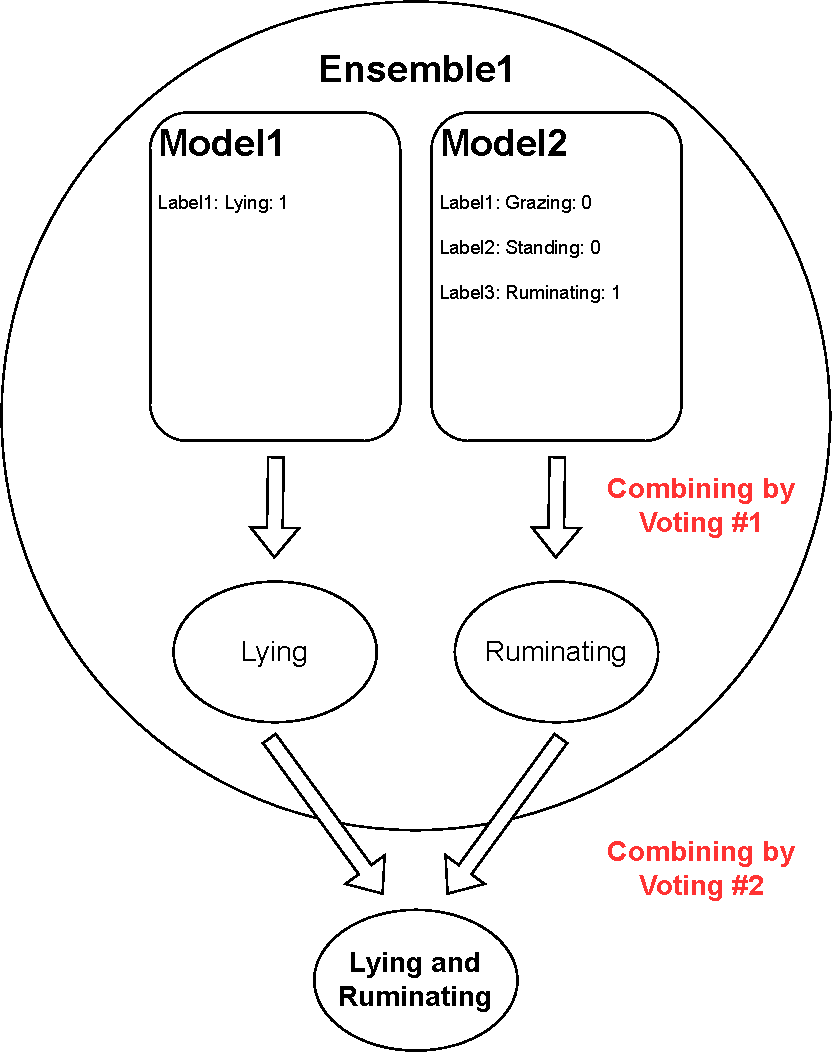
\includegraphics[height=9cm]{graphics/combining.pdf}
      \captionof{figure}{Combining the Classifications Into One Final Label}
      \label{fig:combining}
    \end{minipage}%
    \begin{minipage}{.5\textwidth}
      \centering
      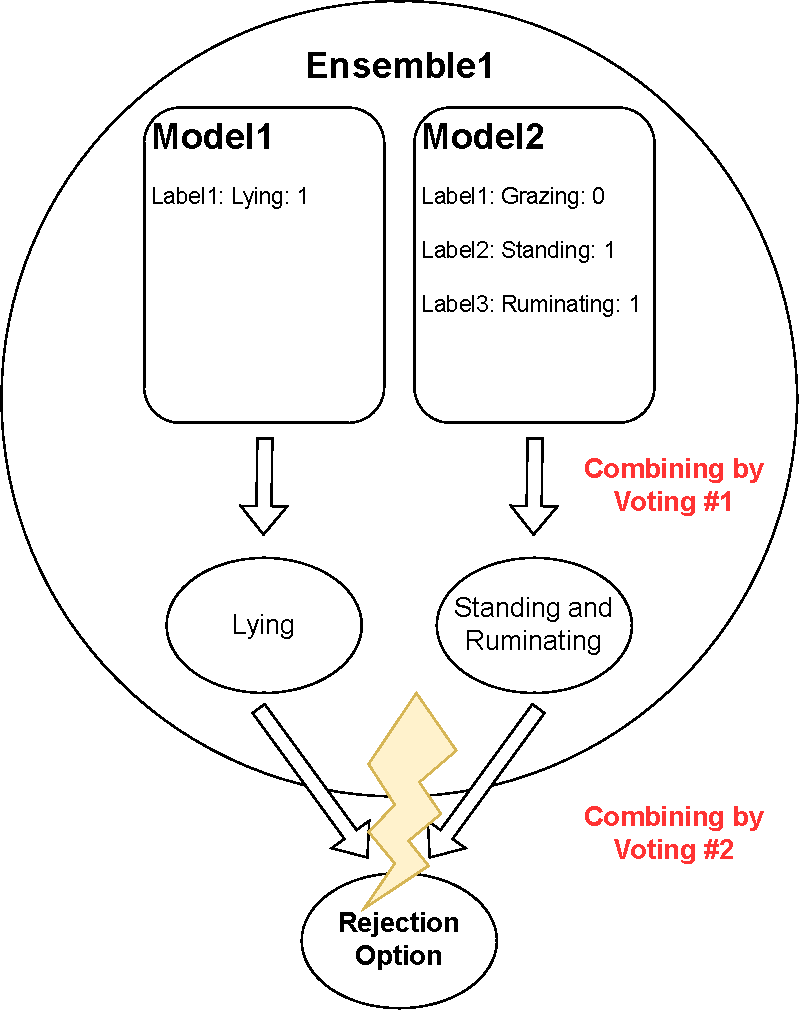
\includegraphics[height=9cm]{graphics/combiningrejection.pdf}
      \captionof{figure}{Rejection Option, As Lying and Standing Are Exclusive Behaviors}
      \label{fig:combiningrejection}
    \end{minipage}
    \end{figure}


Combining the predictions of each classifier brings some crucial benefits to the overall system that impact various aspects of the underlying use case. For one, having displayed only one final result will lead to a much more user-friendly interface. Domain experts or Data Scientists will not have to manually check the prediction of all components of the model set anymore but rather can see the current classification instantly, without having to consider the result of every model on its own. Especially when using larger model sets, the likeliness of errors made by manual human calculation will drop to a minimum. 

During the development stages for this work, it became evident that most ensembles, that were introduced in this section, are not an optimal solution for either use case. Even though some form of voting mechanism is essential for CAR in order to categorize any time interval into one category only, a classic ensemble method like Bagging or Boosting does not seem to be perfectly applicable to this use case. While Stacking seems to be possible for combining the votes for cattle behavior, it comes with expensive resource costs that would contradict the aim of creating a resource-aware system. It must also be noted that combining votes from individual models inside an ensemble is not the focus of this work. Instead, the focus will be on the model selection and retrieval process. Therefore, the outlined approaches regarding combining votes will not be addressed any further. 

Regarding the PAP, predictions from different single models don’t necessarily have to be combined, as they are interpretable and valid on their own. Therefore, a traditional ensemble method would not be relevant for this use case anyway. Instead, a looser combination of different models needed to be created. The implementation that will be introduced in \autoref{chap:implementation} is an attempt to create such combinations. Since the priorly introduced ensemble methods are not entirely practical for PAP and combining votes is not the focus of this work, the term model set will be used to refer to a combination of models from now on. Model sets therefore describe a combination of models whose results do not necessarily need to be combined. Nevertheless, the basic introduction to the topic of ensembles is valuable to gain a deeper understanding of the theoretical foundations of combining machine learning models. As mentioned above, the theoretical concepts, the design, and the implementation that were done for this work mostly refer to the PAP use case. However, the paradigm developed in the course of this work can also be applied to other use cases, in particular the CAR project. 


\section{Resource Awareness} \label{sec:ra}

The following section will give an overview of the topic of resource awareness, by describing it and discussing what metrics could be used to measure resource awareness. In machine learning, resource awareness is applied to various stages of the holistic life cycle of a model. Many previous works \cite{amir2018,tann2016,yu2018} focus on making the inference phase more resource-aware, i.e. reducing the time and computation power needed for the model to produce predictions. Nevertheless, there has since been an increase in making the training process of models more resource-aware as well \cite{rapp2022}.

Resource awareness forms one of the two main pillars this work is focusing on, next to performance. While the two concepts are not necessarily canceling each other out - resource-aware models can definitely be well-performing as well and vice versa - they certainly describe two completely different ideals. This tradeoff between having models that can accurately predict or classify a certain problem, but also making sure that the available resources like memory and computing power are used as efficiently as possible, can generally be solved in one of two ways. One option is to formulate a constrained optimization problem, by defining a limit for a certain measure. An example could be the maximum amount of features a model should use, or the smallest window size one wants to use for preprocessing. The second option is to create a multi-object optimization that aims for an optimal compromise of both relevant measures, i.e. between performance and resource awareness \cite{feurer2019}. As it will become apparent in the following chapters, this work mainly focuses on multi-object optimization by using different weights to level out resource awareness against performance. In addition, however, there will also be an option to use the model set retrieval system as a constrained optimization problem by only creating model sets that use the same feature set.

A central topic of this work was the different stages of measurement of resource awareness. Sünkel et. al. assessed resource awareness using Query Sharing Levels (QSLs) \cite{sunkel2022}. In total, 5 different levels were defined, that describe the extent of properties two or more models share with each other. Each subsequent level is only achievable if the conditions for the previous level are reached. In the mentioned paper, level 0 describes a set of models that have no common qualities. Level 1 is reached, if the models share the same sensor system. If, in addition, the models have undergone the same preprocessing they reach level 2. The third level is reached if the models share the same segmentation (window size), and the highest possible sharing - level 4 - is only reached if the models also have the same features between them. As \autoref{chap:design} will show, the QSLs as proposed in \cite{sunkel2022} have been adjusted for this work. However, the general idea of using different levels to assess the extent of resource awareness between two or more models has been maintained.

By definition, QSLs can only be defined using two or more models. They are not a valid method to evaluate resource awareness on only a single model. This proves to be a rather problematic matter for the case of model set retrieval systems: Only at a late stage in the model set retrieval process, can resource awareness really be considered. A number of model sets have to be created first, in order to look at the extent of resource utilization of those model sets. This means that the learners that make up model sets would either have to be priorly selected based on their performance only (which would result in creating performance-heavy model sets only - the amount of resource-aware model sets could be really low as a result), or every single available model would be used for model set creation (resulting in a very resource costly operation in itself - the vast majority of the created model sets would never be considered in the retrieval process anyway). This problem of having only an option to address resource awareness for model sets and not for single models led to the development of two concepts called inter-model resource awareness and intra-model resource awareness. The extent of efficient resource utilization of a model set is then assessed by looking at that model set from two different perspectives. The main motivation for the development of inter-model and intra-model resource awareness as well as the options that were examined when designing the architecture of the model set retrieval system concerning resource awareness will be provided in \autoref{sec:designretrieval}.


\section{Performance} \label{performance}

The second pillar of this work, next to resource awareness is performance. As performance is a rather broad term and many different metrics can be used to measure the performance of a machine learning model \cite{erickson2021}, some clarification and delimitation of the term has to be made. Generalization performance is a term, that refers to a model's ability to correctly predict new data. It is a crucial point in assessing the quality of a learner and therefore greatly affects the model selection process \cite{hastie2009}. For simplicity, this work will use the term performance when referring to generalization performance. One way to categorize performance metrics is to divide them into four classes which will be introduced shortly: Accuracy-based metrics measure the accuracy of the predicted result in comparison to the true result. Examples of accuracy-based metrics are accuracy in percent, F1, precision, and recall. Error-based metrics on the other hand determine the performance of a model based on the error in prediction between the predicted and the actual value. Mean Absolute Error (MAE), Mean Squared Error (MSE), and Root Mean Squared Error (RMSE) are examples of error-based metrics. Investment-based metrics are of relevance when working with algorithms whose purpose is to come up with investment strategies and usually give context about the risk and reward of a specific strategic approach. Finally, all other informative metrics can be summarized into a miscellaneous category. The metrics of this class usually provide supplementary information that enhances the previously introduced classes of performance metrics \cite{dessain2022}. This work will focus on error- and accuracy-based metrics, namely on accuracy, MAE, MSE, and RMSE.

The idea of using accuracy as a metric of performance seems straightforward, which may be a reason for its popularity in evaluating a machine learning model in the first place. Accuracy provides a general measure of how correctly the model is predicting across the entire dataset. It specifies, with what probability a new data point is predicted correctly \cite{grandini2020}. While this seems very unambiguous for classification problems (either a model predicts the correct behavior of cattle or it doesn’t), there are various things to consider when working in a linear regression setting. If a model would have to predict the occupancy for a parking lot with exact precision (including potential decimal places), probably not many models would have an accuracy value that is considered acceptable. One approach to fix this could be to add a tolerance value when calculating the accuracy of a classifier. If the prediction falls into an interval of $[v-t, v+t]$, where $v$ is the true value and $t$ is the tolerance value, the prediction will be classified as correct. As \autoref{chap:implementation} will show, this approach is applied in this work using the metric \texttt{accuracypercent}. However, the solution that is usually applied for linear regression problems refers to an error-based metric instead, mainly MSE. This way, it can be measured how closely the predicted response value matches the true value for an observation \cite{james2023}. MSE uses a dynamic to have a bigger deviation from the true value increase the error metric exponentially more than smaller deviations. As with all other error-based metrics, a lower score indicates a better-performing model. MSE is calculated using

\begin{equation}
\operatorname{MSE} = \frac{1}{n} \sum_{i=1}^n(y_i - \hat{f}(x_i))^2,
\label{mse}
\end{equation}

where $y_i$ is the true value, and $\hat{f}(x_i)$ is the predicted value.

A similar error-based metric that is widely used for assessing the performance of a model is MAE, which removes the additional penalty for larger deviations from the true value, by averaging the net deviation from the true value without squaring it. It is assessed using 

\begin{equation}
\operatorname{MAE}(y,\hat{y}) = \frac{1}{n} \sum_{i=1}^n |y_i - \hat{y}_i|.
\label{mae}
\end{equation}

Finally, RMSE is used to bring the values of MSE into a usable dimension by taking the square root of MSE. Because of this, the metric is in the same unit as the independent variable, i.e. between 0 and 1 for PAP. Consequently, RMSE is calculated using
\begin{equation}
\operatorname{RMSE} = \sqrt{\frac{1}{n} \sum_{i=1}^n e_t^2 }.
\label{rmse}
\end{equation}


Having defined what performance means in the context of machine learning models, as well as having introduced the metrics for assessing performance in this work, a basic understanding of the two pillars of this project - performance and resource awareness - has been conveyed. 



\section{Top-K Retrieval}\label{sec:topk}

The overall idea of top-k retrieval is straightforward: The user determines a number $k$ of objects they want to receive, and the retrieval algorithm returns the $k$ best items back to the user. As there are numerous variables, settings, and underlying algorithms to consider when using top-k retrieval, the following section will give a brief overview of the topic. 

Before items in a dataset can be assessed for ranking, it must be determined according to what metric(s) those items should be ranked. This is done by using a so-called ranking function, that describes the criteria for the items score that is later used for the actual ranking and selecting of items. A simple ranking function for instance could be the accuracy of a machine learning model. Each model (i.e. item) in the dataset has an assigned accuracy metric in addition to its unique identifier (i.e. primary key). A trivial ranking function could now rank these models according to their accuracy in an ascending or descending order. However, this gets continuously more complicated the more attributes are added to the ranking function: For instance, let us assume that there is another attribute for each machine learning model in the dataset that describes the number of features that were used to train that model. A possible ranking function could now consider both metrics, assigning the model a higher score the higher the accuracy and the lower the number of used features. The general method of ranking the items now is to assess both relevant metrics of an item, apply the ranking function by calculating a score using the (normalized) metrics and optional weights, and ranking every assessed item using this newly computed score. 

A naïve algorithm (NA) would now do this to every item in the database and then output the $k$ items with the highest scores. It is obvious, that such an approach would lead to long retrieval times and computational costs as it would need to consider every single item in the table – even those, that are not nearly close to the top $k$ items. As the costs for this algorithm are linear to the number of total items, it would not be an efficient form of retrieval for databases containing a large number of items \cite{fagin2002}.

Numerous algorithms have been developed in the last decades to utilize a more cost- and time-effective method for top-k retrieval, two of which will be introduced in the following subchapters. A mutuality of those algorithms that is worth examining before going into more detail about their characteristics is the way the data entries are handled: Before the actual calculation of scores can happen, the algorithms first split the database into smaller lists, each containing only two attributes: the relevant attribute that is to be considered for calculation of the score of an item (i.e. performance or resource awareness) and its respective primary key. Therefore, in the example stated above the database would now consist of two lists, one containing the primary key and the accuracy of each model, and the other containing also the primary key in addition to the number of features used to train said model. These lists are then sorted in descending order of the relevant metrics value (and not the primary keys). Consequently, each value gets assigned a grade, depending on its position in the sorted list. The item that has the topmost position in a list therefore has the best grade.

When describing top-k techniques, two types of data access are generally considered that are crucial to understand. The first one is called sorted access and defines obtaining a metric of an object by advancing through the corresponding list sequentially until the according value is reached. Therefore, to access a metric, or score of an item that has the $l^{th}$ best grade in a list, $l$ sorted accesses have to be made in order to obtain this value. NA does $n$ sorted accesses at all times, where $n$ is the number of objects in a list. The other mode of access is called random access. In contrast to sorted access, here the grade of a certain object is identified directly in one step. Instead of having to increment through any other items, the desired grade is accessed immediately. As a drawback, however, random access is often expensive or not even possible in certain scenarios.

With the clarification of these definitions, FA and TA can now be properly introduced.



\subsection{Fagin's Algorithm}

As the name suggests, FA was first introduced by Robert Fagin in 1999 \cite{fagin1999}. Provided that the dataset is already split into separated lists as stated above, an appropriate number $k$ and a scoring function is chosen, the algorithm works as follows:

\begin{enumerate}

\item Sorted access is done to each sorted list in parallel, meaning that first the best-graded metric in each list is accessed, then the second-best metric, and so on. (It is important to understand, that by doing this, not necessarily all metrics of one single object are being accessed at the same time, as an object can have a high grade in one metric, but a rather low one in another metric – which would therefore only be seen after a certain number of sorted accesses in the corresponding list. This sorted access is done until $k$ objects have been seen completely in every list. That means all metrics of at least $k$ objects have been seen through sorted access. 

\item For each object $R$ that has been seen, but not completely seen (meaning at least one grade of $R$ has not been accessed yet), all missing grades from $R$ are accessed through random access. 

\item The overall score is calculated for each object that has been seen using the scoring function. The objects are then sorted by their overall score and finally, the $k$ objects with the highest score are returned. 

\end{enumerate}

It has been proven that under the circumstance of a strict scoring function, FA operates optimally. A scoring function is defined as strict if the overall score of an object reaches its maximum of $1$ when each metric of this object also reaches its maximum value of $1$. However, several situations can be identified, where a scoring function would not behave in a strict manner, for instance when the scoring function is a constant or depicts the maximum value of an object's metrics. In both cases, other algorithms would outperform FA \cite{fagin2002}. Because of such restrictions in the performance of FA, another approach for top-k retrieval shall now be introduced.


\subsection{Threshold Algorithm}

TA first appeared in 2002 after a number of other similar algorithms have been independently developed that aim to solve the same problem \cite{fagin2002a}. Its procedure is as follows:

\begin{enumerate}

\item Much the same as in FA, sorted access is done in parallel in each sorted list. However now, for each seen object $R$, the remaining metrics of $R$ are gathered directly through random access, and $R$'s overall score is calculated using the scoring function. $R$ is stored together with its overall score if it is one of the $k$ highest scores that have been seen yet, breaking ties arbitrarily. 

\item For each sorted access a threshold value is created that consists of calculating an overall score using the metrics that are obtained in this sorted access. In other words, the accessed grades are used to calculate an overall score of a hypothetical object that consists of these accessed grades.  The sorted access is stopped as soon as at least $k$ objects have been seen whose overall score is equal to or higher than the computed threshold value. 

\item The $k$ objects with the highest score that have been stored are returned.

\end{enumerate}
 

 The way the TA is designed, it always has less or equal sorted accesses as FA. In addition, as at most only the $k$ objects with best scores are stored at any time, the required buffer size is noticeably smaller than with FA. The buffer of the latter in contrast can grow quite large as FA remembers every seen object in sorted access \cite{fagin2002}.

% TODO Decide whether or not to include graphics of the algos


\subsection{Additional Top-K Approaches}

Numerous other algorithms have been developed that aim to retrieve the best $k$ items in accordance with a scoring function. Particularly worth mentioning here is the No Random Access algorithm, also developed by Fagin \cite{fagin2002a}. As the name suggests, this algorithm tries to minimize the number of random accesses made to the sorted lists. Overall, all of the top-k processing techniques that focus on the way data is accessed can be summarized into a larger group of top-k methods. However, apart from the way data is accessed, top-k approaches can also be categorized by their proximity to and integration into the underlying database engine \cite{ilyas2008}. Newer approaches, that are characterized by their close relation to the query engine, for instance, include rank-aware query operators or concepts like Group-Ranking \cite{li2006}. Another technique that shall not be unmentioned is the Skyline operator \cite{borzsony2001}. This approach is characterized by not using any form of a scoring function. Instead, multiple objects that dominate other objects in the relevant metrics are returned - similar to a skyline where buildings that are either taller or nearer to the viewer can be seen. It therefore follows that the topmost ranked object for each metric is automatically returned using the Skyline operator. 

While significantly more approaches to top-k retrieval exist \cite{ilyas2008}, the introduced algorithms in this section shall be sufficient for this work. Because of the sheer amount of available top-k methods, the following chapters will focus on the most straightforward and established ones: NA, FA, and TA. The approach of this work will be to compare TA and FA to naïvely retrieving the best $k$ models out of a list. Choosing these data access-based top-k algorithms also has the advantage that the number of accesses can be seen as an indicator for resource awareness. This is why the amount of sorted and random accesses will be one of the evaluation metrics in \autoref{chap:evaluation}. Other methods for ranking objects like the Skyline operator contradict certain relevant points in the introduced use cases, like the idea of having a fixed scoring function. Assessing those miscellaneous top-k approaches therefore goes beyond the scope of this work and will not be further addressed. The advantages of FA and TA will be made apparent by comparing their execution time and the number of accesses to that of NA in \autoref{chap:evaluation}.
With the theoretical foundation having been laid out, the next chapters, however, will first be dedicated to the practical sides of the model retrieval process by introducing the development done for this work.